%% Exercice 2

%\ExoSpecs{\TTBF{CalculTVA.sh}}{\TTBF{\RenduDir/src/exo1/}}{750}{640}{\TTBF{write}}
\ExoSpecsCustom{\TTBF{stack\_linked\_list.c}}{\TTBF{\RenduDir/src/}}{750}{640}{Fonctions autorisées}{\TTBF{malloc(3)}, \TTBF{free(3)}, \TTBF{memcpy(3)}, \TTBF{printf(3)}}

\vspace*{0.7cm}

\noindent \ExoObjectif{Le but de l'exercice est d'implémenter une pile en C à base de liste chaînée.}

\bigskip

%\noindent Les fonctions demandées dans cet exercice devront se trouver dans une bibliothèque nommée \TTBF{libmystack}.
%Après un appel à la commande \texttt{make} à la racine du projet, il faut que votre chaîne de compilation produise à la racine de votre projet une version statique de la bibliothèque (qui se nommera \TTBF{libmystack.a}) ainsi qu'une version dynamique de la bibliothèque (qui se nommera \TTBF{libmystack.so}).
%
%\bigskip

\noindent Vous devez écrire plusieurs fonctions permettant de créer, utiliser, vider, et libérer une pile.
Un fichier \TTBF{stack\_linked\_list.h} contenant toutes les fonctions exportables à implémenter vous est fourni en annexe.
Vous devez déclarer une structure \TTBF{stack\_ll} et l'ajouter dans \TTBF{stack\_linked\_list.h}.
N'oubliez pas de déclarer également une structure qui contiendra les éléments de la liste chaînée.
Pour les premières étapes, vous devrez implémenter une version simplifiée de la pile qui ne prend en charge que des entiers positifs.

\bigskip

\noindent Conceptuellement, les fonctions manipulant des piles de type \TTBF{stack\_ll*} devront pouvoir gérer ces 3 cas :

\bigskip

\begin{center}
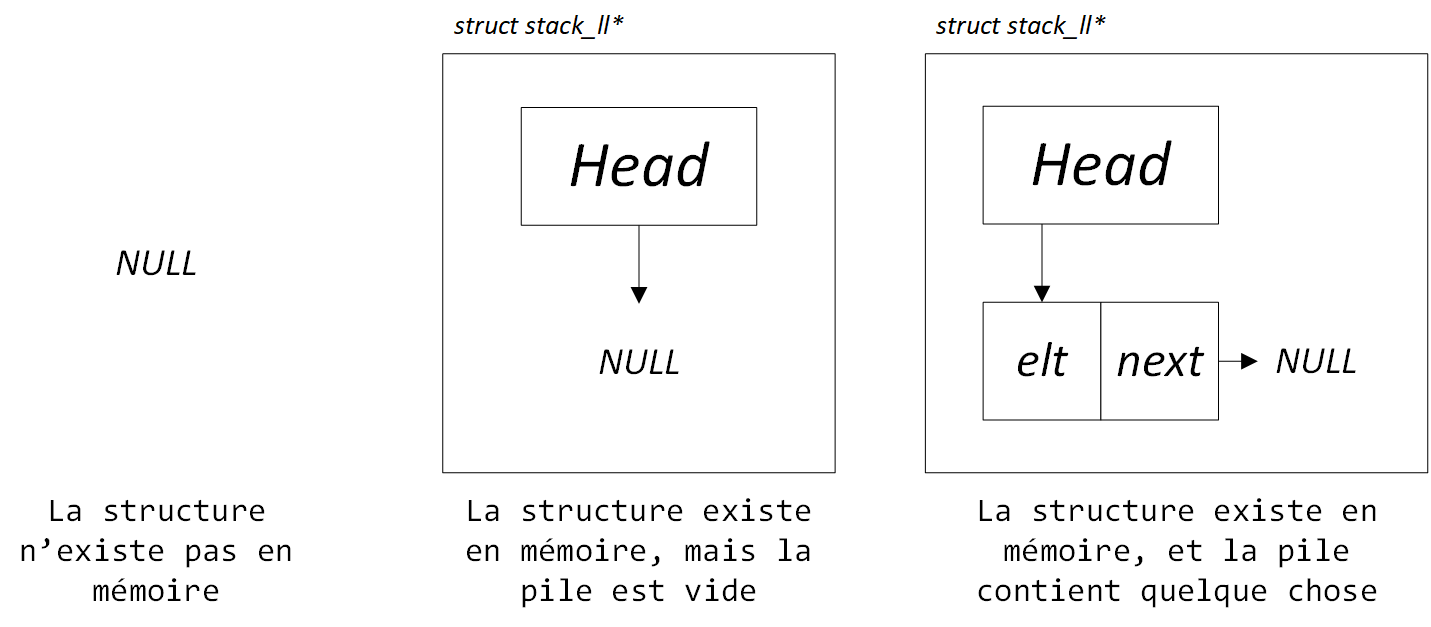
\includegraphics[scale=0.85]{Cours/Piles_Implementation_LL.png}
\end{center}

%\bigskip
\newpage

%\noindent Vous devez implémenter les 11 fonctions suivantes :
%\begin{itemize}
%\item \TTBF{stack\_ll *stack\_ll\_create(void)}
%\item \TTBF{void stack\_ll\_delete(stack\_ll *stack)}
%\item \TTBF{int stack\_ll\_length(stack\_ll *stack)}
%\item \TTBF{int stack\_ll\_push(int elt, stack\_ll *stack)}
%\item \TTBF{int stack\_ll\_pop(stack\_ll *stack)}
%\item \TTBF{int stack\_ll\_head(stack\_ll *stack)}
%\item \TTBF{int stack\_ll\_clear(stack\_ll *stack)}
%\item \TTBF{int stack\_ll\_is\_empty(stack\_ll *stack)}
%\item \TTBF{int stack\_ll\_search(int elt, stack\_ll *stack)}
%\item \TTBF{stack\_ll *stack\_ll\_reverse(stack\_ll *stack)}
%\item \TTBF{void stack\_ll\_print(stack\_ll *stack)}
%\end{itemize}

\noindent Vous devez implémenter les fonctions suivantes :

\bigskip

\lstset{language=C}
\begin{lstlisting}[frame=single,title={Liste des fonctions pour une pile avec liste chaînée}]
stack_ll *stack_ll_create(void);
void stack_ll_delete(stack_ll *stack);

int stack_ll_length(stack_ll *stack);

int stack_ll_push(int elt, stack_ll *stack);
int stack_ll_pop(stack_ll *stack);
int stack_ll_head(stack_ll *stack);

int stack_ll_clear(stack_ll *stack);
int stack_ll_is_empty(stack_ll *stack);

int stack_ll_search(int elt, stack_ll *stack);
stack_ll *stack_ll_reverse(stack_ll *stack);
void stack_ll_print(stack_ll *stack);
\end{lstlisting}


\subsubsection*{\TTBF{stack\_ll *stack\_ll\_create(void)}}

\noindent Cette fonction crée une pile vide.
En cas d'erreur (pas assez de mémoire), elle renvoie un pointeur \TTBF{NULL}.


\subsubsection*{\TTBF{void stack\_ll\_delete(stack\_ll *stack)}}

\noindent Cette fonction vide une pile de l'ensemble de ses éléments, et détruit la structure restante.
Si le paramètre donné est \TTBF{NULL}, la fonction ne fait rien.


\subsubsection*{\TTBF{int stack\_ll\_length(stack\_ll *stack)}}

\noindent Cette fonction renvoie la longueur de la pile (c'est-à-dire le nombre d'éléments actuellement dans la pile).
Si le paramètre donné est \TTBF{NULL}, la fonction renvoie $ -1 $.


\subsubsection*{\TTBF{int stack\_ll\_push(int elt, stack\_ll *stack)}}

\noindent Cette fonction empile un élément dans une pile, c'est-à-dire qu'elle ajoute un élément au sommet.
En cas de succès, la fonction renvoie $ 0 $.
Si la pile donnée en paramètre est \TTBF{NULL}, la fonction renvoie $ -1 $.
Si le nombre donné en paramètre est inférieur à $ 0 $, la fonction renvoie $ -4 $.
S'il y a un problème de mémoire, la fonction renvoie $ -3 $.


\subsubsection*{\TTBF{int stack\_ll\_pop(stack\_ll *stack)}}

\noindent Cette fonction dépile un élément d'une pile, c'est-à-dire qu'elle supprime l'élément au sommet.
En cas de succès, la fonction renvoie $ 0 $.
Si la pile donnée en paramètre est \TTBF{NULL}, la fonction renvoie $ -1 $.
Si la pile donnée en paramètre est vide, la fonction renvoie $ -2 $.


\subsubsection*{\TTBF{int stack\_ll\_head(stack\_ll *stack)}}

\noindent Cette fonction renvoie l'élément au sommet de la pile.
Si la pile donnée en paramètre est \TTBF{NULL}, la fonction renvoie $ -1 $.
Si la pile donnée en paramètre est vide, la fonction renvoie $ -2 $.


\subsubsection*{\TTBF{int stack\_ll\_clear(stack\_ll *stack)}}

\noindent Cette fonction vide une pile de l'ensemble de ses éléments, sans détruire la structure de la pile.
La fonction renvoie le nombre d'éléments supprimés de la mémoire.
Si le paramètre donné est \TTBF{NULL}, la fonction renvoie $ -1 $.
Si la pile donnée en paramètre est vide, la fonction renvoie $ 0 $.


\subsubsection*{\TTBF{int stack\_ll\_is\_empty(stack\_ll *stack)}}

\noindent Cette fonction teste si une pile est vide ou non.
Si la pile est vide, la fonction renvoie $ 1 $.
Si la pile n'est pas vide, la fonction renvoie $ 0 $.
Si la pile donnée en paramètre est \TTBF{NULL}, la fonction renvoie $ -1 $.


\subsubsection*{\TTBF{int stack\_ll\_search(int elt, stack\_ll *stack)}}

\noindent Cette fonction recherche un élément dans la pile et renvoie sa position dans la liste chaînée.
La première position est celle où l'élément le plus ancien a été placé (c'est-à-dire le fond de la pile), cette position sera numérotée $ 0 $.
Si l'élément n'est pas trouvé, la fonction renvoie $ -4 $.
Si la pile donnée en paramètre est \TTBF{NULL}, la fonction renvoie $ -1 $.


\subsubsection*{\TTBF{stack\_ll *stack\_ll\_reverse(stack\_ll *stack)}}

\noindent Cette fonction inverse la position de tous les éléments de la pile.
Le premier élément devient le dernier, l'avant dernier devient le deuxième, etc.
En cas de succès, la fonction renvoie le pointeur vers l'éventuelle nouvelle adresse en mémoire de la structure de la pile inversée.
En cas de problème mémoire, on renvoie \TTBF{NULL}, et l'ancienne pile doit rester à son ancienne adresse mémoire sans subir la moindre modification.
Si la pile donnée en paramètre est \TTBF{NULL}, la fonction renvoie \TTBF{NULL}.


\subsubsection*{\TTBF{void stack\_ll\_print(stack\_ll *stack)}}

\noindent Cette fonction affiche le contenu de la pile.
Le format d'affichage attendu implique d'afficher un seul élément par ligne, suivi d'un retour à la ligne.
L'élément en tête de pile sera affiché en premier.
Si la pile donnée en paramètre est vide, seul un retour à la ligne est affiché.
Si la pile donnée en paramètre est \TTBF{NULL}, rien n'est affiché.

\bigskip

\lstset{language=sh}
\begin{lstlisting}[frame=single,title={Exemple d'affichage du cas normal : pile contenant 42, 5, 13}]
$ ./my_stack_linked_list
42
5
13

$
\end{lstlisting}

\bigskip

\lstset{language=sh}
\begin{lstlisting}[frame=single,title={Exemple d'affichage d'une pile vide}]
$ ./my_stack_linked_list

$
\end{lstlisting}

\bigskip

\lstset{language=sh}
\begin{lstlisting}[frame=single,title={Exemple d'affichage d'un pointeur NULL}]
$ ./my_stack_linked_list
$
\end{lstlisting}
